

	
\section{Il problema di De Saint Venant}	
	Il modello alla De Saint Venant si propone di ricavare deformazioni e tensioni su di un oggetto ideale, a partire dai carichi esterni opportunamente applicati. 
	
	Si ipotizzeranno delle soluzioni che sostituite nel problema porteranno al soddisfacimento delle ipotesi (metodo inverso): partendo dalle ipotesi di De Saint Venant, si ipotizzerà una soluzione, se questa sostituita nelle ipotesi di partenza le soddisferà, allora la soluzione sarà esatta, ed esistendo, per il principio di Kirchhoff, sarà l'unica. \newline
	
\subsection{Ipotesi semplificative}
\begin{figure}[H]
	\centering
	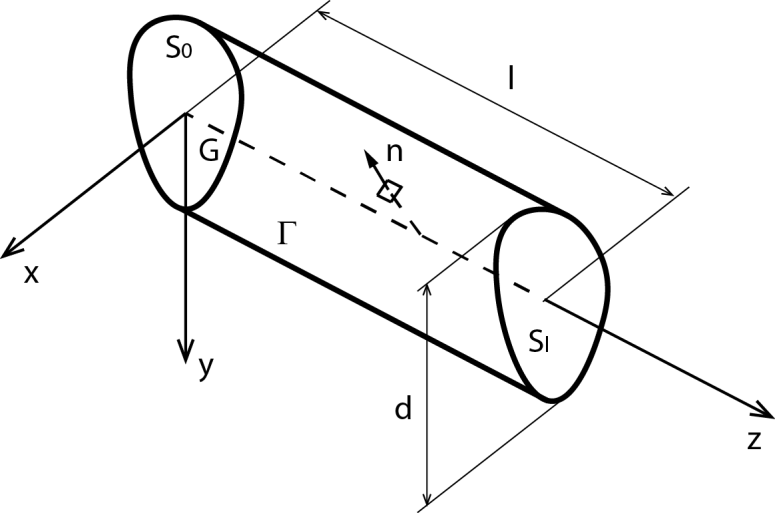
\includegraphics[width=0.5\linewidth]{Immagini_2/screenshot001}
	\label{fig:screenshot001}
\end{figure}
	\begin{enumerate}
	\item \textbf{Ipotesi sulla geometria}:
		\begin{itemize}		
		\item La dimensione caratteristica (ingombro massimo di sezione) della sezione retta della trave
		deve risultare trascurabile rispetto alla sua lunghezza $ d/l<<1 $: la trave dev'essere snella, non tozza;
		\item La trave è ad asse rettilineo;
		\item Sezioni rette costanti lungo z;
		\end{itemize}

	\item \textbf{Ipotesi sui carichi esterni}:
		\begin{itemize}
			\item  Le forze di volume $ f $ sono nulle, si ignora la forza peso;
		\item Le forze di superfici	$ p $ sono applicate solo sulle basi e non sulla superficie laterale;
		\item Il sistema si trova in equilibrio;
		\item Il corpo è libero da vincoli, trascuro ovvero i carichi da questi generati all'interno delle caratteristiche della sollecitazione;
		\end{itemize}
	\item \textbf{Ipotesi sul materiale costitutivo}:
		\begin{itemize}
			\item Materiale elastico lineare e isotropo (due parametri per caratterizzarlo: Young e Poisson);
		\item La trave è omogenea, ovvero le caratteristiche del	materiale non variano da punto a punto
		\end{itemize}
	\end{enumerate}
	Con un sistema di riferimento baricentrico con $z$ asse della trave. \newline 
	
	\textbf{Equazioni indefinite di equilibrio}:
\[ \text{in} ~ \Omega
\begin{cases}
	\begin{aligned}
		\frac{\partial\sigma_x}{\partial x} + \frac{\partial \tau_{yx}}{\partial y} + \frac{\partial \tau_{zx}}{\partial z} & =0 \\
		
		\frac{\partial \tau_{xy}}{\partial x} + \frac{\partial\sigma_y}{\partial y} + \frac{\partial \tau_{zy}}{\partial z} & =0 \\
		
		\frac{\partial \tau_{xz}}{\partial x} + \frac{\partial \tau_{yz}}{\partial y} + \frac{\partial\sigma_z}{\partial z} & =0 \\
	\end{aligned}
\end{cases}
\]

	\textbf{Equazioni al contorno:} 
\[
\text{in} ~ \Sigma \begin{cases}
	p_x = \sigma_x n_x + \tau_{yx}n_y + \tau_{zx}n_z \\
	p_y = \tau_{xy}n_x + \sigma_y n_y + \tau_{zy}n_z \\
	p_z = \tau_{xz}n_x + \tau_{yz}n_y + \sigma_z n_z \\
\end{cases}
\]
\[
\text{mantello} ~ (n_x,n_y,0) \begin{cases}
\sigma_x n_x + \tau_{yx}n_y =0 \\
\tau_{xy}n_x + \sigma_y n_y =0 \\
\tau_{xz}n_x + \tau_{yz}n_y =0 \\
\end{cases} 
\]
\[
\text{$S_0$} ~ (0,0,-1) ~ \begin{cases}
	\tau_{zx} = -p_x \\
	\tau_{zy} = -p_y \\
	\sigma_z = -p_z \\
\end{cases}
\hspace{0.5cm}
\text{$S_l$} ~ (0,0,1) ~ \begin{cases}
	\tau_{zx} = p_x \\
	\tau_{zy} = p_y \\
	\sigma_z = p_z \\
\end{cases}
\]

\textbf{Legame costitutivo:}
\[ [\varepsilon] = [C][\sigma]\]

	\textbf{Equazioni di congruenza:}
\[ 
\begin{cases}
	\begin{aligned}
		\varepsilon_{xx} =   \frac{\partial u_x}{\partial x} \\
		\varepsilon_{yy} =   \frac{\partial u_y}{\partial y} \\
		\varepsilon_{zz} =   \frac{\partial u_z}{\partial z} \\
	\end{aligned}
\end{cases} \hspace{1cm} \begin{cases}
	\begin{aligned}
		\gamma_{xy} =   \frac{\partial u_y}{\partial x} + \frac{\partial u_x}{\partial y} \\
		\gamma_{yz} =   \frac{\partial u_y}{\partial z} + \frac{\partial u_z}{\partial y} \\
		\gamma_{zx} =   \frac{\partial u_z}{\partial x} + \frac{\partial u_x}{\partial z} \\
	\end{aligned}
\end{cases}
\]
\begin{figure}[H]
	\centering
	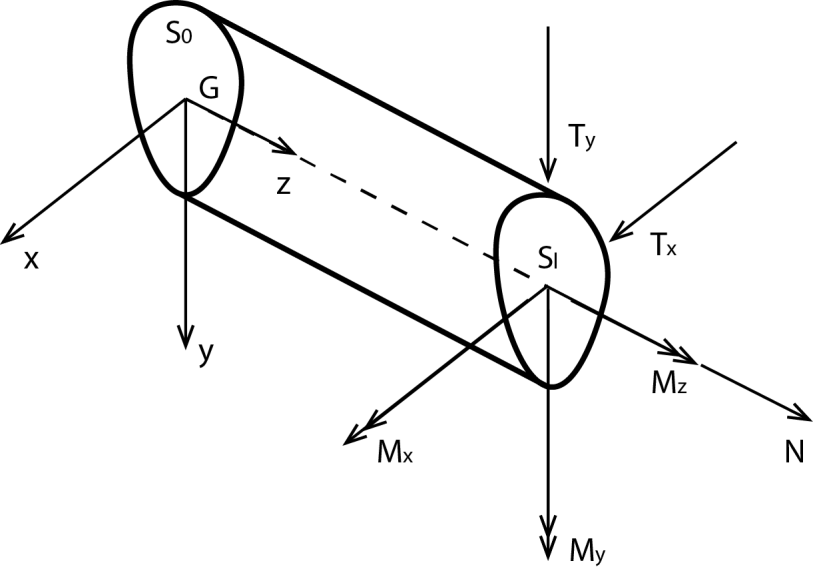
\includegraphics[width=0.5\linewidth]{Immagini_2/screenshot002}
	\label{fig:screenshot002}
\end{figure}
Ottengo così un set di equazioni per cui si ipotizzerà una soluzione che si dovrà verificare in queste equazioni per controllare che siano tutte rispettate. \newline 

È necessario tradurre le sollecitazioni in tensioni: servono le caratteristiche della sollecitazione. 
\begin{itemize}
	\item[$\rightarrow$] La risultante dello \textbf{sforzo normale}? È la risultante delle azioni in direzione $z$; 
\item[$\rightarrow$] La risultante dello \textbf{sforzo di taglio}? È la risultante delle rispettive azioni sull'asse $x$ e sull'asse $y$
\item[$\rightarrow$] Come si genera il momento intorno all'asse $x$? $P_x$ e $P_y$ giacciono in $xy$ e quindi non hanno braccio per generare una rotazione intorno ad $x$, l'unica azione che può farlo è $P_z$.
\item[$\rightarrow$] Il \textbf{momento intorno all'asse $y$} sarà generato come appena detto, introducendo un segno $-$ dovuto alla convenzione della regola della mano destra. 
\item[$\rightarrow$] Ed il \textbf{momento intorno a $z$}? È un momento torcente. 

L'azione di un momento torcente porta alla spostamento in direzione $x$ degli elementi infinitesimi della sezione e non genera spostamento sull'asse baricentrico. 

È generato da $P_x$ e $P_y$ e non da $P_z$, questo parallelo a $z$. 

Il segno è dato in base al fatto che gli elementi infinitesimi soggetti a $P_x$ e distanti $y$ sono negativi, mentre quelli soggetti a $P_y$ e distanti $x$ sono positivi, sempre in accordo con la regola della mano destra. 
\end{itemize}


\begin{figure}[H]
	\centering
	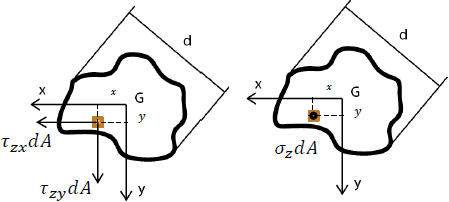
\includegraphics[width=0.5\linewidth]{Immagini_2/screenshot003}
	\label{fig:screenshot003}
\end{figure}

	Adesso, attraverso le equazioni di equilibrio al contorno, si possono legare le tensioni alle deformazioni, le caratteristiche della sollecitazione sulla $S_l$ perciò saranno:
\[\begin{matrix}
	\begin{aligned}
		N = \int_A P_zdA = \int_A \sigma_zdA  \hspace{1cm} & M_x = \int_A P_zydA = \int_A \sigma_zydA  \\
		T_x = \int_A P_xdA = \int_A \tau_{zx}dA \hspace{1cm} &  M_y = -\int_A P_zxdA = -\int_A \sigma_zxdA \\
		T_y = \int_A P_ydA = \int_A \tau_{zy}dA \hspace{1cm} &  M_z = \int_A (\tau_{zy}x -\tau_{zx}y)dA
	\end{aligned}	
\end{matrix}\]
	

	Il problema si riduce così alla determinazione dello stato tensionale a partire dalla conoscenza dell'equilibrio delle caratteristiche della sollecitazione. 

	Sapendo inoltre che le equazioni trovate sono valide per una sezione del materiale, essendo questo LOI per ipotesi, varranno per tutto il materiale. \newline

   \begin{en} [\textbf{Principio di De SaintVenant}]
		Se ad un elemento superficiale di un solido è applicato un sistema di forze autoequilibrato, lo stato di tensione nei punti del solido a sufficiente distanza dall’elemento caricato è praticamente nullo (distanza di estinzione).
	\end{en}  
	
	Ne consegue che, se si applica alla base dell'elemento trave un sistema di forze autoequilibrato, ad una certa distanza da tale base lo stato di tensione non dipende dalla
	distribuzione dei carichi effettivi applicati sulle basi ma soltanto dalle caratteristiche della sollecitazione. \newline	
	
	La distanza a cui l’effetto dei carichi in equilibrio sulle basi diventa nullo è detta distanza di estinzione e risulta in genere pari alla dimensione massima $ d $ della sezione retta.\newline 
	
	Per cui se si determina lo stato tensionale interno per una distribuzione particolare delle sollecitazioni superficiali
	sulle basi allora si è in grado di determinare lo stato tensionale per una qualsiasi distribuzione con le
	stesse caratteristiche. \newline 
	
	Come si scrive il tensore delle tensioni di De Saint Venant? 
	
	Le caratteristiche della sollecitazione varieranno lungo l'asse per cui in ogni punto dell'asse varrà una mappatura di tensioni lungo la sezione. \newline	
	 
	In questo caso sulla base sono presenti 3 tensioni: 
	\begin{equation}
	\boxed{[\sigma] = \left[ \begin{array}{ccc}
		0 & 0 & \tau_{xz} \\
		0 & 0 & \tau_{yz} \\
		\tau_{zx} & \tau_{zy} & \sigma_z
	\end{array}\right]}
	\end{equation} 
	Le soluzioni di questo tensore delle tensioni sono dette soluzioni alla De Saint Venant. \newline 

	Come si comporta la trave di De Saint Venant?
	
	Fisicamente equivale a considerare la trave come un insieme di fibre longitudinali \textit{spaghettiformi} che trasferiscono
	azioni mutue tangenzialmente alla direzione delle fibre stesse.  
	\begin{figure}[H]
		\centering
		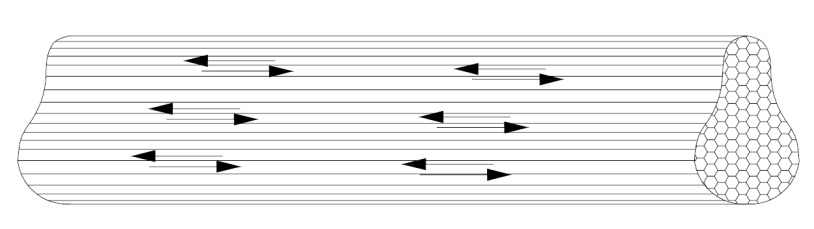
\includegraphics[width=0.5\linewidth]{Immagini_2/screenshot004}
		\label{fig:screenshot004}
	\end{figure}	
	
\begin{itemize}
	\item[$\Rightarrow$] Le equazioni indefinite di equilibrio diventano: 
	\[ \begin{cases}
		\begin{aligned}
			\frac{\partial \tau_{zx}}{\partial z} & =0 \\
			
			\frac{\partial \tau_{zy}}{\partial z} & =0 \\
			
			\frac{\partial \tau_{xz}}{\partial x} + \frac{\partial \tau_{yz}}{\partial y} + \frac{\partial\sigma_z}{\partial z} & =0 \\
		\end{aligned}
	\end{cases}\]
	Dalle prime due equazioni si deriva che il vettore delle tensioni $\vec{\tau}_z=(\tau_{xz},\tau_{yz})$ risulta costante in $ z $ e quindi indipendente da $ z $, ovvero su di un piano ortogonale a $z$ agisce un campo vettoriale del tipo:
	\[ \vec{\tau}_z=\tau_{xz}(x,y)\hat{i} + \tau_{yz}(x,y)\hat{j} \]
	Per ottenere la tensione normale si derivi la terza equazioni in $z$:
	\[\frac{\partial^2 \tau_{xz}}{\partial x\partial z} + \frac{\partial^2 \tau_{yz}}{\partial y\partial z} + \frac{\partial^2\sigma_z}{\partial^2 z}  = 0 \]
	\[ \frac{\partial^2\sigma_z}{\partial^2 z}  = 0 \Rightarrow \frac{\partial\sigma_z}{\partial z}  = cost \]
	\[ \sigma_z (x,y,z)= \dfrac{z}{l}\sigma_z (x,y,z) + \dfrac{l-z}{l}\sigma_z (x,y,z)\]
	$\sigma_z$ è lineare, lungo la fibra varia linearmente. \newline


	\item[$\Rightarrow$] Quello a cui ci si riconduce è uno stato tensionale piano: ridotto il tensore delle tensioni ad un tensore principale, ovvero se delle infinite terne disponibili ci si limita a quelle principali, se i 3 pivot sono non nulli lo stato di tensione è tridimensionale, se uno è nullo lo stato sarà bidimensionale e se due sono nulli lo stato sarà monodimensionale. \newline 

	Le direzioni principali si ricavano dal tensore delle tensioni generico ponendo il determinale pari a zero, nel caso di De Saint Venant: 
	\[ \det[\sigma] \equiv 0 \]
	Esistono allora sicuramente almeno due soluzioni non nulle, il problema sarà così definibile piano.
	
	Poiché lo stato tensionale è piano, il piano delle tensioni sarà individuato dal vettore della tensione tangenziale $\tau$ e dal vettore della tensione normale $\sigma$, da cui ne consegue il fatto che i punti della stessa fibra avranno lo stesso piano delle tensioni: lungo lo spaghetto $\tau_{xz}, \tau_{yz}$ sono costanti, ma non è detto che non possano variare nelle altre direzioni. \newline
	
	Quali sono a questo punto le direzioni principali? Una sarà data da $z$, l'altra da $\tau$ e la terza verrà ricavata di conseguenza. 
\end{itemize}
		
\section{Forza Normale Centrata}
	Si cerchi una soluzione al problema applicando la più semplice delle sollecitazioni, una tensione monodimensionale per cui la risultante delle forze esterne applicate sulle basi estremali sia equivalente ad una forza centrata N:
	\[ \begin{cases}
		p_x =0 \\
		p_y = 0 \\
		p_z = c
	\end{cases} \hspace{1cm} \begin{cases}
	\tau_{xz} = p_x = 0 \\
	\tau_{yz} = p_y = 0 \\
	\sigma_z = p_z = c
\end{cases}\]
	Ne derivano le seguenti caratteristiche della sollecitazione:
	\[\begin{matrix}
		\begin{aligned}
			N = \int_A \sigma_zdA = cA \hspace{1cm} & M_z = \int_A (\tau_{zy}x -\tau_{zx}y)dA = 0 \\
			T_x = \int_A \tau_{zx}dA = 0 \hspace{1cm} & M_x = \int_A \sigma_zydA = c\int_A ydA = cS_x  \\
			T_y = \int_A \tau_{zy}dA = 0 \hspace{1cm} & M_y = -\int_A \sigma_zxdA = -c\int_A zxdA = -cS_y
		\end{aligned}	
	\end{matrix}\]
 	Dove con $S_x, S_y$ si sono identificati i momenti statici, questi nulli se - come per ipotesi - ci si è posti in un sistema di riferimento baricentrale.  (Ricordi la geometria delle aree?) \newline
 	
 	La sollecitazione si configura così essere semplicemente di sforzo normale solo se l’asse $ z $ è baricentrico per la trave.
 	\begin{figure}[H]
 		\centering
 		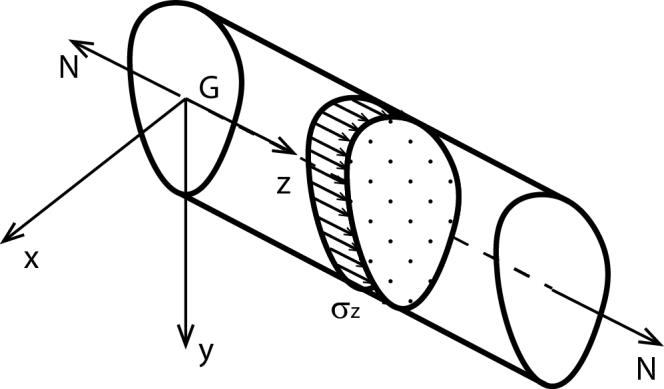
\includegraphics[width=0.5\linewidth]{Immagini_2/screenshot005}
 		\label{fig:screenshot005}
 	\end{figure}	
 	Si integrino le condizioni di equilibrio, in $z$: $\begin{cases}
 		\tau_{zx} = cost \\
 		\tau_{zy} = cost 
 	\end{cases}$ \newline per definizione le tensioni agli estremi sono nulle (è applicata solo N) e dunque \newline $\tau_{zx} = \tau_{zy} = 0 ~ \forall z  \in  (0,l)$ queste, sostituite nella terza equazione di equilibrio portano a:
 \[ \dfrac{\partial\sigma_z}{\partial z} = 0 \Rightarrow \sigma_z = cost ~ \text{in $z$}\] 
 	Poiché in $z=l$ la tensione è nota:
 \[ 	N = \int_A \sigma_zdA = cA \]
	 Ma è noto che: \[ \sigma_z = c\] Allora:  \[N  = \sigma_zA \Rightarrow \sigma_z = \frac{N}{A} \] Verificando la forma del tensore delle tensioni per stato tensionale monoassiale:
 \begin{equation}
 \boxed{	\left[ \begin{array}{ccc}
 	0 & 0 & 0 \\
 	0 & 0 & 0 \\
 	0 & 0 & \dfrac{N}{A}
 \end{array}\right]} 
 \end{equation}
 	Ricordi che la terna principale è una terna di assi per la quale il tensore delle
 	tensioni è una matrice diagonale? In questo caso essendo la matrice diagonale, si conclude che la terna principale sarà così formata dall'asse $z$ e da qualsiasi altri assi che siano ortogonali a $z$ e tra di loro. \newline
\begin{itemize}
	 	
 \item[$\Rightarrow$] Si valutino a questo punto la congruenza ed il legame costituivo, condensati questi nelle relazioni di Navier, integrando queste equazioni si può così risalire agli spostamenti in maniera univoca.
 	\[ 
 \begin{cases}
 	\begin{aligned}
 		\varepsilon_{xx} =   \frac{\partial u_x}{\partial x} = \dfrac{1}{E}[\sigma_x - \nu(\sigma_y + \sigma_z)] = -\dfrac{\nu N}{EA} \\
 		\varepsilon_{yy} =   \frac{\partial u_y}{\partial y} = \dfrac{1}{E}[\sigma_y - \nu(\sigma_x + \sigma_z)] = -\dfrac{\nu N}{EA} \\
 		\varepsilon_{zz} =   \frac{\partial u_z}{\partial z} = \dfrac{1}{E}[\sigma_z - \nu(\sigma_x + \sigma_y)] = \dfrac{ N}{EA} \\
 	\end{aligned}
 \end{cases} \hspace{1cm} \begin{cases}
 	\begin{aligned}
 		\gamma_{xy} =   \frac{\partial u_y}{\partial x} + \frac{\partial u_x}{\partial y} = \dfrac{1}{G} \tau_{xy} = 0\\
 		\gamma_{yz} =   \frac{\partial u_y}{\partial z} + \frac{\partial u_z}{\partial y} = \dfrac{1}{G} \tau_{xz} = 0 \\
 		\gamma_{zx} =   \frac{\partial u_z}{\partial x} + \frac{\partial u_x}{\partial z} = \dfrac{1}{G} \tau_{yz} = 0 \\
 	\end{aligned}
 \end{cases}
 \]
 	Ricordi che $EA$ è il modulo di rigidezza? \newline 
 	
 	 Quali sono i risultati notevoli? Innanzitutto si nota subito che a seguito di una trazione che c'è un allungamento in direzione $z$ dato da $\varepsilon_{zz} = \dfrac{ N}{EA}$ e una diminuzione di sezione (strizione!) lungo $ x $ e lungo $ y $ data dai contributi $\varepsilon_{xx} = \varepsilon_{yy} = -\dfrac{\nu N}{EA}$, si nota infine  la più totale assenza di distorsioni, i termini in $\gamma$ sono tutti nulli, in questo modo la sezione NON si modificherà, non cambiando gli angoli tra le rette/fibre. 
 	
 	\item[$\Rightarrow$] Adesso ci si pone di analizzare gli spostamenti associati a questo tipo di sforzo normale centrato: si integreranno le equazioni di Navier appena scritte.
 \[ \begin{cases}
 	\begin{aligned}
 	u & = -\dfrac{\nu N}{EA}x + u_0(z,y) \\
 	v & = -\dfrac{\nu N}{EA}y + v_0(z,x) \\
 	w & = \dfrac{N}{EA}z + w_0(x,y)
 	\end{aligned}
 \end{cases} \]
	Si ottengono così degli spostamenti definiti a meno di funzioni, se queste funzioni descrivono un moto che non dà contributi in termini direzionali deformativi, il corpo si muoverà nello spazio senza subire ulteriori tensioni e deformazioni compiendo un \textbf{moto rigido} e queste funzioni potranno essere trascurate. 
	
	Si sostituiscano perciò tali funzioni all'interno delle equazioni degli allungamenti e distorsioni:
		\[ 
	\begin{cases}
		\begin{aligned}
			\varepsilon_{0x} =   \frac{\partial u_0}{\partial x} = 0 \\
			\varepsilon_{0y} =   \frac{\partial v_0}{\partial y} = 0 \\
			\varepsilon_{zz} =   \frac{\partial w_0}{\partial z} = 0 \\
		\end{aligned}
	\end{cases} \hspace{1cm} \begin{cases}
		\begin{aligned}
			\gamma_{0xy} =   \frac{\partial u_0}{\partial x} + \frac{\partial u_0}{\partial y} = 0\\
			\gamma_{0yz} =   \frac{\partial v_0}{\partial z} + \frac{\partial w_0}{\partial y} =  0 \\
			\gamma_{0zx} =   \frac{\partial w_0}{\partial x} + \frac{\partial u_0}{\partial z} =  0 \\
		\end{aligned}
	\end{cases}
	\]
	Come ci si poneva di dimostrare a tali funzioni non sono associati nè allungamenti nè distorsioni, perciò sono caratteristiche di un moto rigido. \newline
	
	Gli spostamenti sono così infine definiti a meno di un moto rigido:
	\begin{equation}		 
	\boxed{	\begin{cases}
		\begin{aligned}
			u & = -\dfrac{\nu N}{EA}x  \\
			v & = -\dfrac{\nu N}{EA}y  \\
			w & = \dfrac{N}{EA}z 
		\end{aligned}
	\end{cases}}
	\end{equation}

\end{itemize}
	In conclusione, lo sforzo normale genera una trasformazione omotetica del solido, ovvero una variazione di volume ma non di forma in base al segno di $N$:
	\[ \begin{cases}
		N>0 ~ \text{Trazione, aumento di volume} \\
		N<0 ~ \text{Compressione, diminuzione di volume}
	\end{cases}
	\]
	Rimanendo sempre nel campo di sollecitazioni elastiche,
	per $ N>0 $ il volume aumenta, c'è di mezzo un modulo di Poisson, la trave si allunga di più di quanto si strizioni, le fibre longitudinali si allungano più di quanto non si
	accorcino quelle trasversali: i punti sul mantello si avvicinano al baricentro rendendo tuttavia la configurazione deformata affine a quella indeformata è per questo che la variazione di volume è comunque positiva: l’asse baricentrico viene allungato in direzione $ z $, al contrario delle altre fibre longitudinali che subiscono
	anche una strizione (avvicinamento all’asse baricentrico).
	
	Per la compressione $ N<0 $ invece, la trave si comprime assialmente più di quanto si allunghi lateralmente. \newline
	
	L'entità dello spostamento delle fibre è proporzionale alla quota $xy$: la strizione diviene maggiore allontanandosi dalla zona centrale. \newline
	
	Inoltre la sezione retta resta tale spostandosi su di un piano parallelo cambiando però forma:
	\[ x' = x + u = x \left(1-\dfrac{\nu N}{EA}\right) \hspace{1cm } y' = y + v = y \left(1-\dfrac{\nu N}{EA}\right) \hspace{1cm } z' = z + w = w \left(1-\dfrac{ N}{EA}\right)\]
	
